\subsubsection{\Glspl{flexion-image}}\label{flexion-image-section}

Each pixel of a \Gls{flexion-image} is the dot-product of the local normal
calculated from horizontal and vertical neighbouring pixel with the
normal calculated with the diagonal neighbours.
Figure~\ref{fig:flexion-image-scetched} demonstrates the disparity of both normals for an arbitrary surface patch.
The normal calculated from the diagonal and vertical neighbouring vertices are drawn in blue and the normal calculated with the diagonals red.
Both normal-vectors are drawn with their origin in the central depth value.

\begin{figure}[H]
    \begin{subfigure}[t]{0.49\linewidth}
        \centering
        \scalebox{1.0}{%
        

\tikzset{every picture/.style={line width=0.75pt}} %set default line width to 0.75pt        

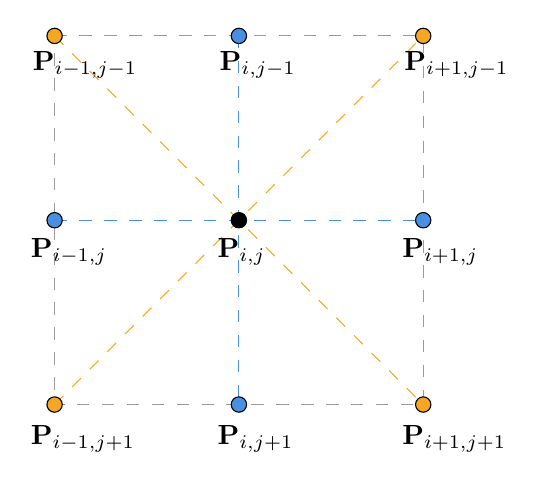
\begin{tikzpicture}[x=0.75pt,y=0.75pt,yscale=-1,xscale=1]
%uncomment if require: \path (0,237); %set diagram left start at 0, and has height of 237

%Shape: Rectangle [id:dp6565487036659107] 
\draw  [color={rgb, 255:red, 155; green, 155; blue, 155 }  ,draw opacity=1 ][dash pattern={on 4.5pt off 4.5pt}] (28.7,13.7) -- (206.3,13.7) -- (206.3,191.3) -- (28.7,191.3) -- cycle ;
%Straight Lines [id:da30195081571029425] 
\draw [color={rgb, 255:red, 74; green, 144; blue, 226 }  ,draw opacity=1 ] [dash pattern={on 4.5pt off 4.5pt}]  (28.7,102.5) -- (206.3,102.5) ;
%Straight Lines [id:da4586174781414081] 
\draw [color={rgb, 255:red, 74; green, 144; blue, 226 }  ,draw opacity=1 ] [dash pattern={on 4.5pt off 4.5pt}]  (117.5,13.7) -- (117.5,191.3) ;
%Straight Lines [id:da7294828306266232] 
\draw [color={rgb, 255:red, 245; green, 166; blue, 35 }  ,draw opacity=1 ] [dash pattern={on 4.5pt off 4.5pt}]  (28.7,13.7) -- (206.3,191.3) ;
%Straight Lines [id:da3243995266948473] 
\draw [color={rgb, 255:red, 245; green, 166; blue, 35 }  ,draw opacity=1 ] [dash pattern={on 4.5pt off 4.5pt}]  (28.7,191.3) -- (206.3,13.7) ;
%Shape: Circle [id:dp5266363779447065] 
\draw  [fill={rgb, 255:red, 245; green, 166; blue, 35 }  ,fill opacity=1 ] (25,13.7) .. controls (25,11.66) and (26.66,10) .. (28.7,10) .. controls (30.74,10) and (32.4,11.66) .. (32.4,13.7) .. controls (32.4,15.74) and (30.74,17.4) .. (28.7,17.4) .. controls (26.66,17.4) and (25,15.74) .. (25,13.7) -- cycle ;
%Shape: Ellipse [id:dp14497174740803043] 
\draw  [fill={rgb, 255:red, 74; green, 144; blue, 226 }  ,fill opacity=1 ] (25,102.5) .. controls (25,100.46) and (26.66,98.8) .. (28.7,98.8) .. controls (30.74,98.8) and (32.4,100.46) .. (32.4,102.5) .. controls (32.4,104.54) and (30.74,106.2) .. (28.7,106.2) .. controls (26.66,106.2) and (25,104.54) .. (25,102.5) -- cycle ;
%Shape: Ellipse [id:dp0427609892023727] 
\draw  [fill={rgb, 255:red, 245; green, 166; blue, 35 }  ,fill opacity=1 ] (25,191.3) .. controls (25,189.26) and (26.66,187.6) .. (28.7,187.6) .. controls (30.74,187.6) and (32.4,189.26) .. (32.4,191.3) .. controls (32.4,193.34) and (30.74,195) .. (28.7,195) .. controls (26.66,195) and (25,193.34) .. (25,191.3) -- cycle ;
%Shape: Ellipse [id:dp2872052196845898] 
\draw  [fill={rgb, 255:red, 74; green, 144; blue, 226 }  ,fill opacity=1 ] (113.8,13.7) .. controls (113.8,11.66) and (115.46,10) .. (117.5,10) .. controls (119.54,10) and (121.2,11.66) .. (121.2,13.7) .. controls (121.2,15.74) and (119.54,17.4) .. (117.5,17.4) .. controls (115.46,17.4) and (113.8,15.74) .. (113.8,13.7) -- cycle ;
%Shape: Circle [id:dp758793708555806] 
\draw  [fill={rgb, 255:red, 0; green, 0; blue, 0 }  ,fill opacity=1 ] (113.8,102.5) .. controls (113.8,100.46) and (115.46,98.8) .. (117.5,98.8) .. controls (119.54,98.8) and (121.2,100.46) .. (121.2,102.5) .. controls (121.2,104.54) and (119.54,106.2) .. (117.5,106.2) .. controls (115.46,106.2) and (113.8,104.54) .. (113.8,102.5) -- cycle ;
%Shape: Circle [id:dp477059334030714] 
\draw  [fill={rgb, 255:red, 74; green, 144; blue, 226 }  ,fill opacity=1 ] (113.8,191.3) .. controls (113.8,189.26) and (115.46,187.6) .. (117.5,187.6) .. controls (119.54,187.6) and (121.2,189.26) .. (121.2,191.3) .. controls (121.2,193.34) and (119.54,195) .. (117.5,195) .. controls (115.46,195) and (113.8,193.34) .. (113.8,191.3) -- cycle ;
%Shape: Ellipse [id:dp13207731000753575] 
\draw  [fill={rgb, 255:red, 245; green, 166; blue, 35 }  ,fill opacity=1 ] (202.6,13.7) .. controls (202.6,11.66) and (204.26,10) .. (206.3,10) .. controls (208.34,10) and (210,11.66) .. (210,13.7) .. controls (210,15.74) and (208.34,17.4) .. (206.3,17.4) .. controls (204.26,17.4) and (202.6,15.74) .. (202.6,13.7) -- cycle ;
%Shape: Circle [id:dp8288145253462365] 
\draw  [fill={rgb, 255:red, 74; green, 144; blue, 226 }  ,fill opacity=1 ] (202.6,102.5) .. controls (202.6,100.46) and (204.26,98.8) .. (206.3,98.8) .. controls (208.34,98.8) and (210,100.46) .. (210,102.5) .. controls (210,104.54) and (208.34,106.2) .. (206.3,106.2) .. controls (204.26,106.2) and (202.6,104.54) .. (202.6,102.5) -- cycle ;
%Shape: Circle [id:dp9160642610677009] 
\draw  [fill={rgb, 255:red, 245; green, 166; blue, 35 }  ,fill opacity=1 ] (202.6,191.3) .. controls (202.6,189.26) and (204.26,187.6) .. (206.3,187.6) .. controls (208.34,187.6) and (210,189.26) .. (210,191.3) .. controls (210,193.34) and (208.34,195) .. (206.3,195) .. controls (204.26,195) and (202.6,193.34) .. (202.6,191.3) -- cycle ;

% Text Node
\draw (106,110) node [anchor=north west][inner sep=0.75pt]   [align=left] {$\displaystyle \mathbf{P}_{i,j}$};
% Text Node
\draw (195,110) node [anchor=north west][inner sep=0.75pt]   [align=left] {$\displaystyle \mathbf{P}_{i+1,j}$};
% Text Node
\draw (16,110) node [anchor=north west][inner sep=0.75pt]   [align=left] {$\displaystyle \mathbf{P}_{i-1,j}$};
% Text Node
\draw (107,20) node [anchor=north west][inner sep=0.75pt]   [align=left] {$\displaystyle \mathbf{P}_{i,j-1}$};
% Text Node
\draw (196,20) node [anchor=north west][inner sep=0.75pt]   [align=left] {$\displaystyle \mathbf{P}_{i+1,j-1}$};
% Text Node
\draw (17,20) node [anchor=north west][inner sep=0.75pt]   [align=left] {$\displaystyle \mathbf{P}_{i-1,j-1}$};
% Text Node
\draw (106,200) node [anchor=north west][inner sep=0.75pt]   [align=left] {$\displaystyle \mathbf{P}_{i,j+1}$};
% Text Node
\draw (195,200) node [anchor=north west][inner sep=0.75pt]   [align=left] {$\displaystyle \mathbf{P}_{i+1,j+1}$};
% Text Node
\draw (16,200) node [anchor=north west][inner sep=0.75pt]   [align=left] {$\displaystyle \mathbf{P}_{i-1,j+1}$};


\end{tikzpicture}


        }
        \caption{The normals for a point $\mathbf{P_{i,j}}$ can be estimated its diagonal or horizontal and vertical neighbours.}
    \end{subfigure}
    \begin{subfigure}[t]{0.49\linewidth}
        \centering
        \begin{tikzpicture}
    \node[anchor=south west,inner sep=0] (image) at (4.0,0) {\includegraphics[width=0.6\textwidth]{chapter04/img/flexion-model-2-clipped.png}};
    \node at (4.4, 5.1) {$\mathbf{P_{i-1,j-1}}$};
    \node at (6.2, 5.5) {$\mathbf{P_{i,j-1}}$};
    \node at (8.5, 5.8) {$\mathbf{P_{i+1,j-1}}$};

    \node at (4.7, 2.9) {\scalebox{0.9}{$\mathbf{P_{i-1,j}}$}};
    \node at (6.2, 2.5) {$\mathbf{P_{i,j}}$};
    \node at (7.7, 3.0) {$\mathbf{P_{i+1,j}}$};

    \node at (5.0, 0.9) {$\mathbf{P_{i-1,j+1}}$};
    \node at (6.3, 0.4) {$\mathbf{P_{i,j+1}}$};
    \node at (9.2, 0.3) {$\mathbf{P_{i+1,j+1}}$};

    \node [plotdarkblue] at (4.6, 3.5) {$\vec{n_1}$};
    \node [plotdarkorange] at (4.8, 2.3) {$\vec{n_2}$};
\end{tikzpicture}

        \caption{The estimated normals span an angle depending on the local shape of the surface measured by the depth sensors.}
    \end{subfigure}
    \caption[Schematic Representation of Flexion]{This figure demonstrates how flexed surfaces have different normals for diagonal and non-diagonal estimation. This difference is utilized as measure for flexion.}%
    \label{fig:flexion-image-scetched}
\end{figure}

The flexion $f$ is defined as
\begin{align}
    f &= \abs{n_1 \cdotp n_2}
\end{align}
Because $n_1$ and $n_2$ are of length $1$ the value of $f$ is in the range $[0, 1]$ and gets scaled accordingly.

The smaller the dot-product gets, the higher is the local flexion of the
surface. This local property of the geometry then results in visual
features detectable with classical feature detectors and descriptors like
\Gls{sift} or \Gls{surf}.
